\section{Modellering af Semplito og dets komponenter}
\label{kabitel:ModelleringSystem}
\subsection{Designklassediagram(DCD)}
\label{DCD}

For at bedre overskue associationerne mellem klasserne i vores program, samt for at give et overblik over hvilke metoder klasserne har, har vi lavet et DCD. 

DCD'et er baseret på vores objekt- og domænemodel, se afsnit \ref{objektmodel} og \ref{domaenemodel} og er blevet opdateret løbende i projektet.
DCD'et har været med til at sikre, at kodestandarden blev overholdt.
Dertil har det gjort det nemmere at bestemme ansvaret for hver klasse.

Når man laver et DCD er det vigtigt, at kravene til programmet repræsenteres, så det bliver implementeret rigtigt.
Med det menes, at en metodes signatur skal også indeholde hvilke variabeltyper den modtager og returnere, at metoder og variables tilgængelighed skal kunne ses, det skal vises, hvis en klasse arver fra en anden klasse eller implementere et interface.
Det skal også vises, hvilke klasser kender til hinanden ved at bruge associationspile.

For at holde det overskueligt har vi både lavet et samlet DCD, men også lavet mindre DCD'er, der er bundet til en bestemt use case, og derfor kun indeholder de klasser, som er relevante for use casen.

På figur \ref{fig:DCD} kan domænelaget af DCD'en for use casen: Book Ny Aftale ses.
I bilagene på figurene \ref{bilag:RelationDCD}, \ref{bilag:UIDCD}, \ref{bilag:ApplicationDCD}, \ref{bilag:DomainDCD}, \ref{bilag:PersistableDCD} kan en samlet DCD for hele systemet ses.

% Mangler evt. noget mere om hvordan den er blevet holdt op til programmet. also pictures

\begin{sidewaysfigure}
    \caption{DCD for Semplito - Bookingsystemet}
    \centering
        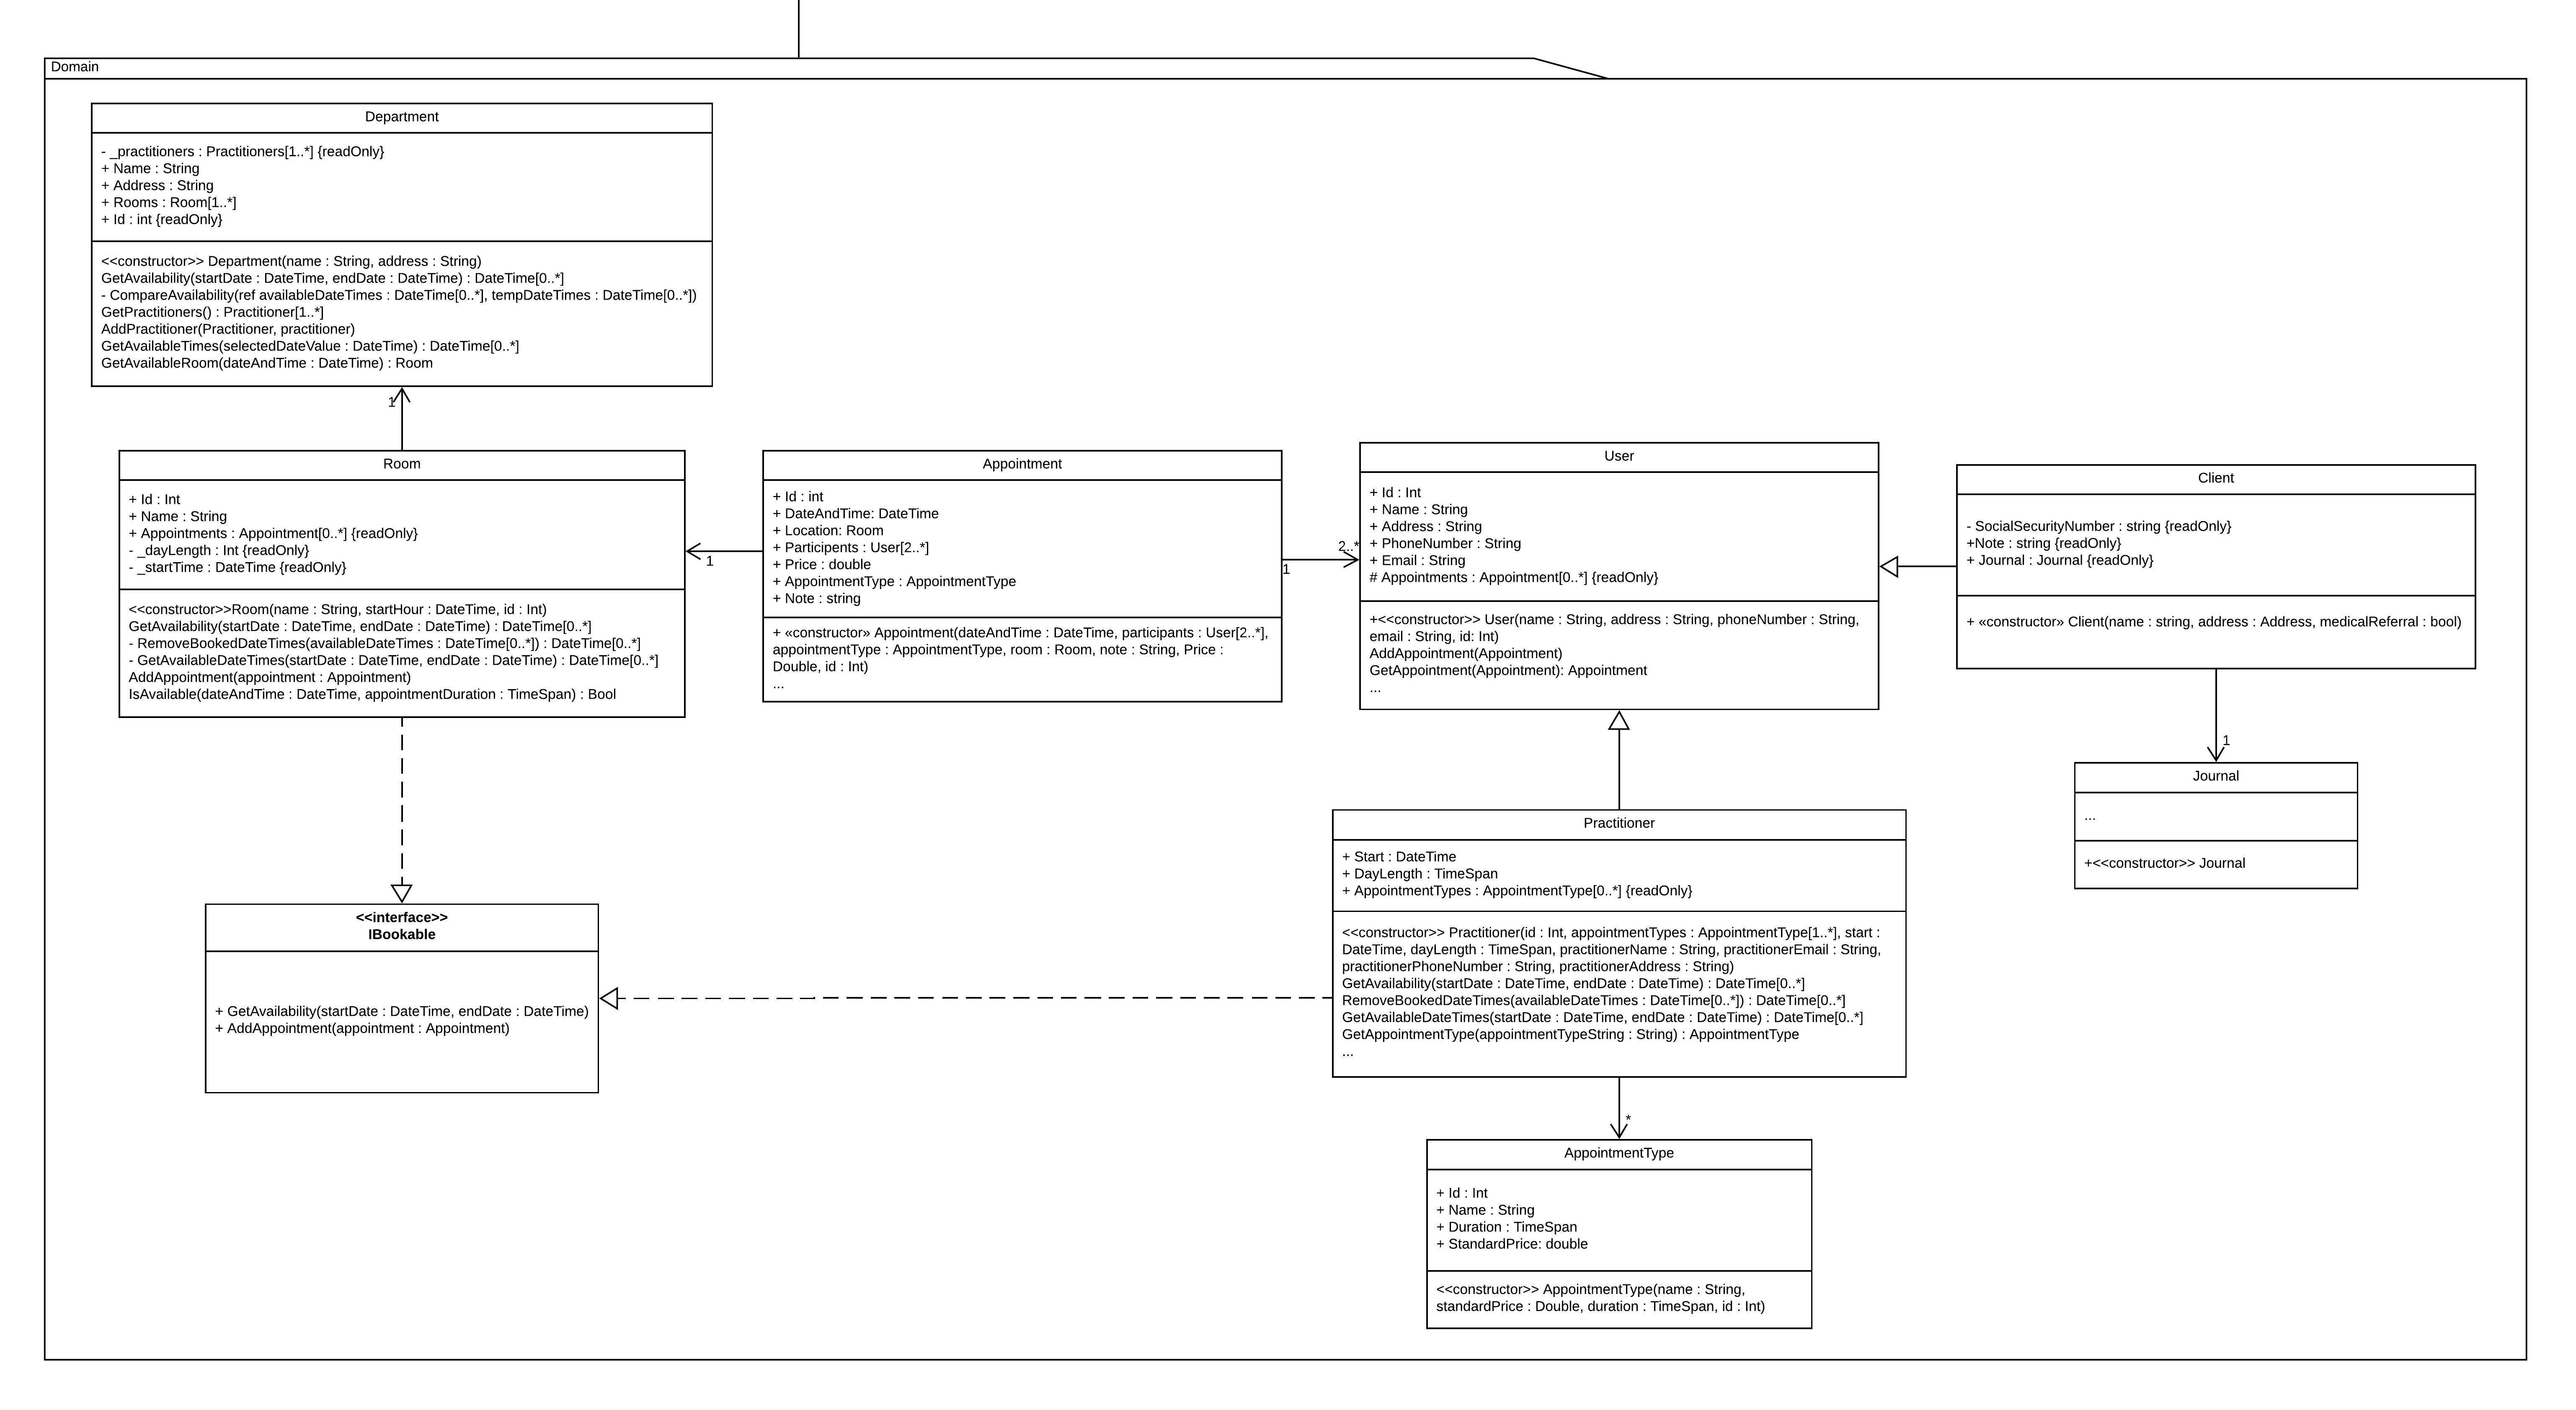
\includegraphics[width=\textwidth]{DomainDCD.png}
    \label{fig:DCD}
\end{sidewaysfigure}

\subsection{Sekvensdiagram(SD)}
\label{SD}

Et SD beskriver, hvordan softwareklasser taler sammen.
Det er vigtigt, at SD'et derfor er på samme sprog, som man ønsker ens kode skal være, da metodenavnene i SD'et er de metoder, som udvikleren implementerer.
Derfor skal metoderne også være de samme metoder, som i ens DCD.

På figur \ref{fig:SD} kan et SD for SOC'en createAppointment ses.
Når en bruger trykker på opret aftale knappen i opret aftale vinduet, vil vinduet kalde controlleren, som kalder videre ned i systemet til appointmentRepo objektet, der laver en ny aftale, og tilføjer referencer til det nye aftale objekt i det angivne room objekt og de angivne user objekter.
Til sidst kalder appointmentRepo objektet sit IPersistable objekt.

\begin{sidewaysfigure}
    \caption{SD for SOC Operation - createAppointment}
    \centering
        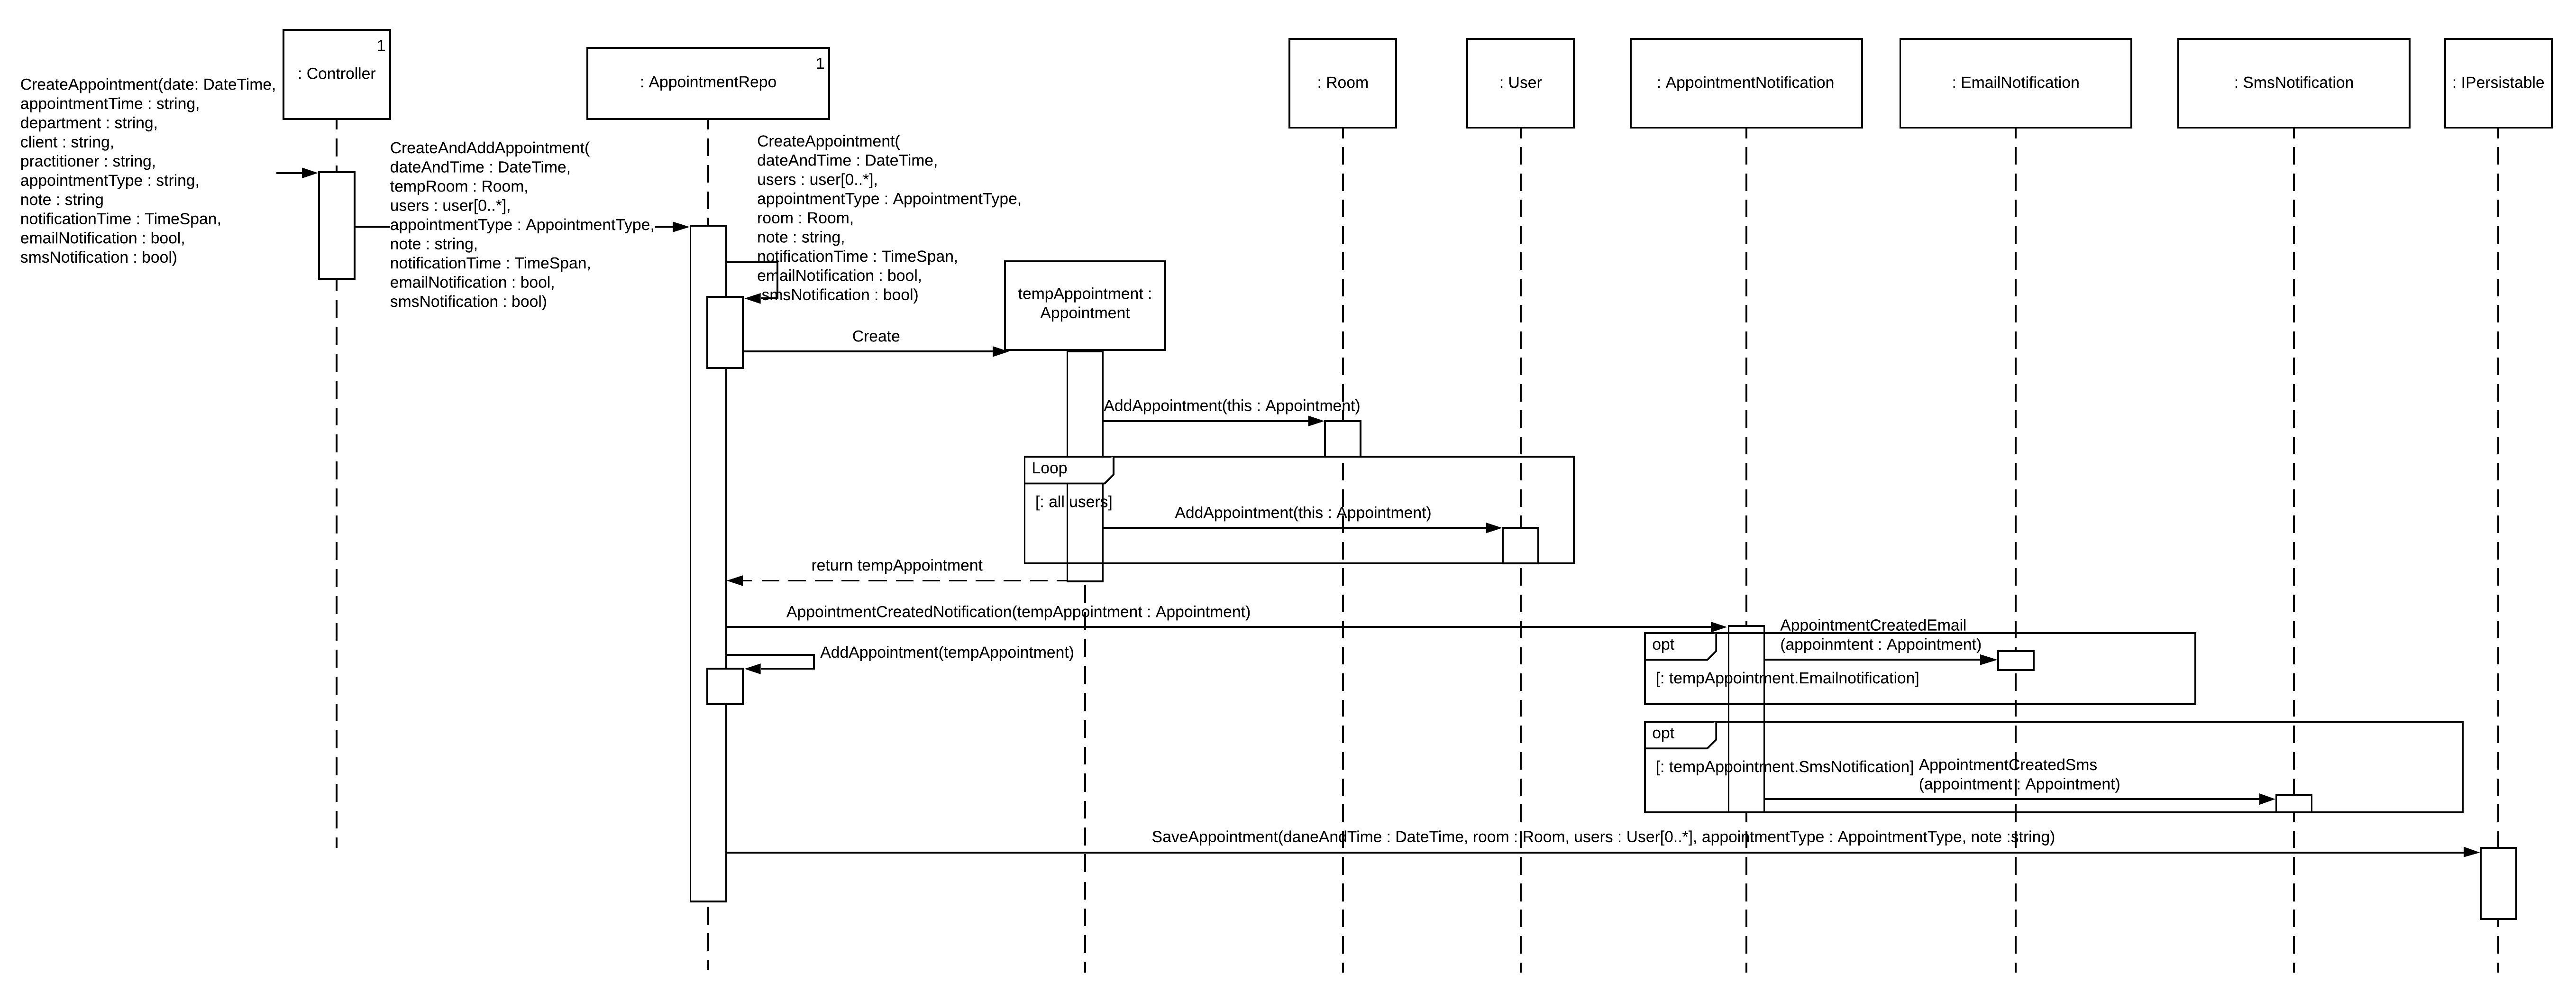
\includegraphics[width=\textwidth]{SD.png}
    \label{fig:SD}
\end{sidewaysfigure}

\subsection{Pakkediagram - Lagdeling}
\label{Pakkediagram}

Ud over vores DCD lavede vi også et pakkediagram.
Pakkediagrammet er til stor hjælp, når man skal finde rundt i programmets forskellige klasser og lag.
Ligesom DCD'et kan det give et overblik over hvilke klasser, der har kendskab til hinanden, men uden at vise metoderne, som kan gøre det sværere at overskue relationerne mellem de forskellige klasser.
Samtidigt viser pakkediagrammet mere omkring programmets lagdeling, da klasserne er opdelt i de lag, som vi har opdelt vores system i, se figur \ref{fig:pakkediagram}.

Pakkediagrammet giver os et bedre overblik over programmet som helhed, hvor DCD'et giver mulighed for at kigge nærmere på klasserne.

Både pakkediagrammet og DCD'et har været brugt i mange gode diskussioner i gruppen, i forbindelse med vores valg af softwarearkitektur.
Vores valg af lagdeling vil blive diskuteret nærmere i afsnit \ref{lagdeling}.

\begin{sidewaysfigure}
    \caption{Pakkediagram for systemet}
    \centering
        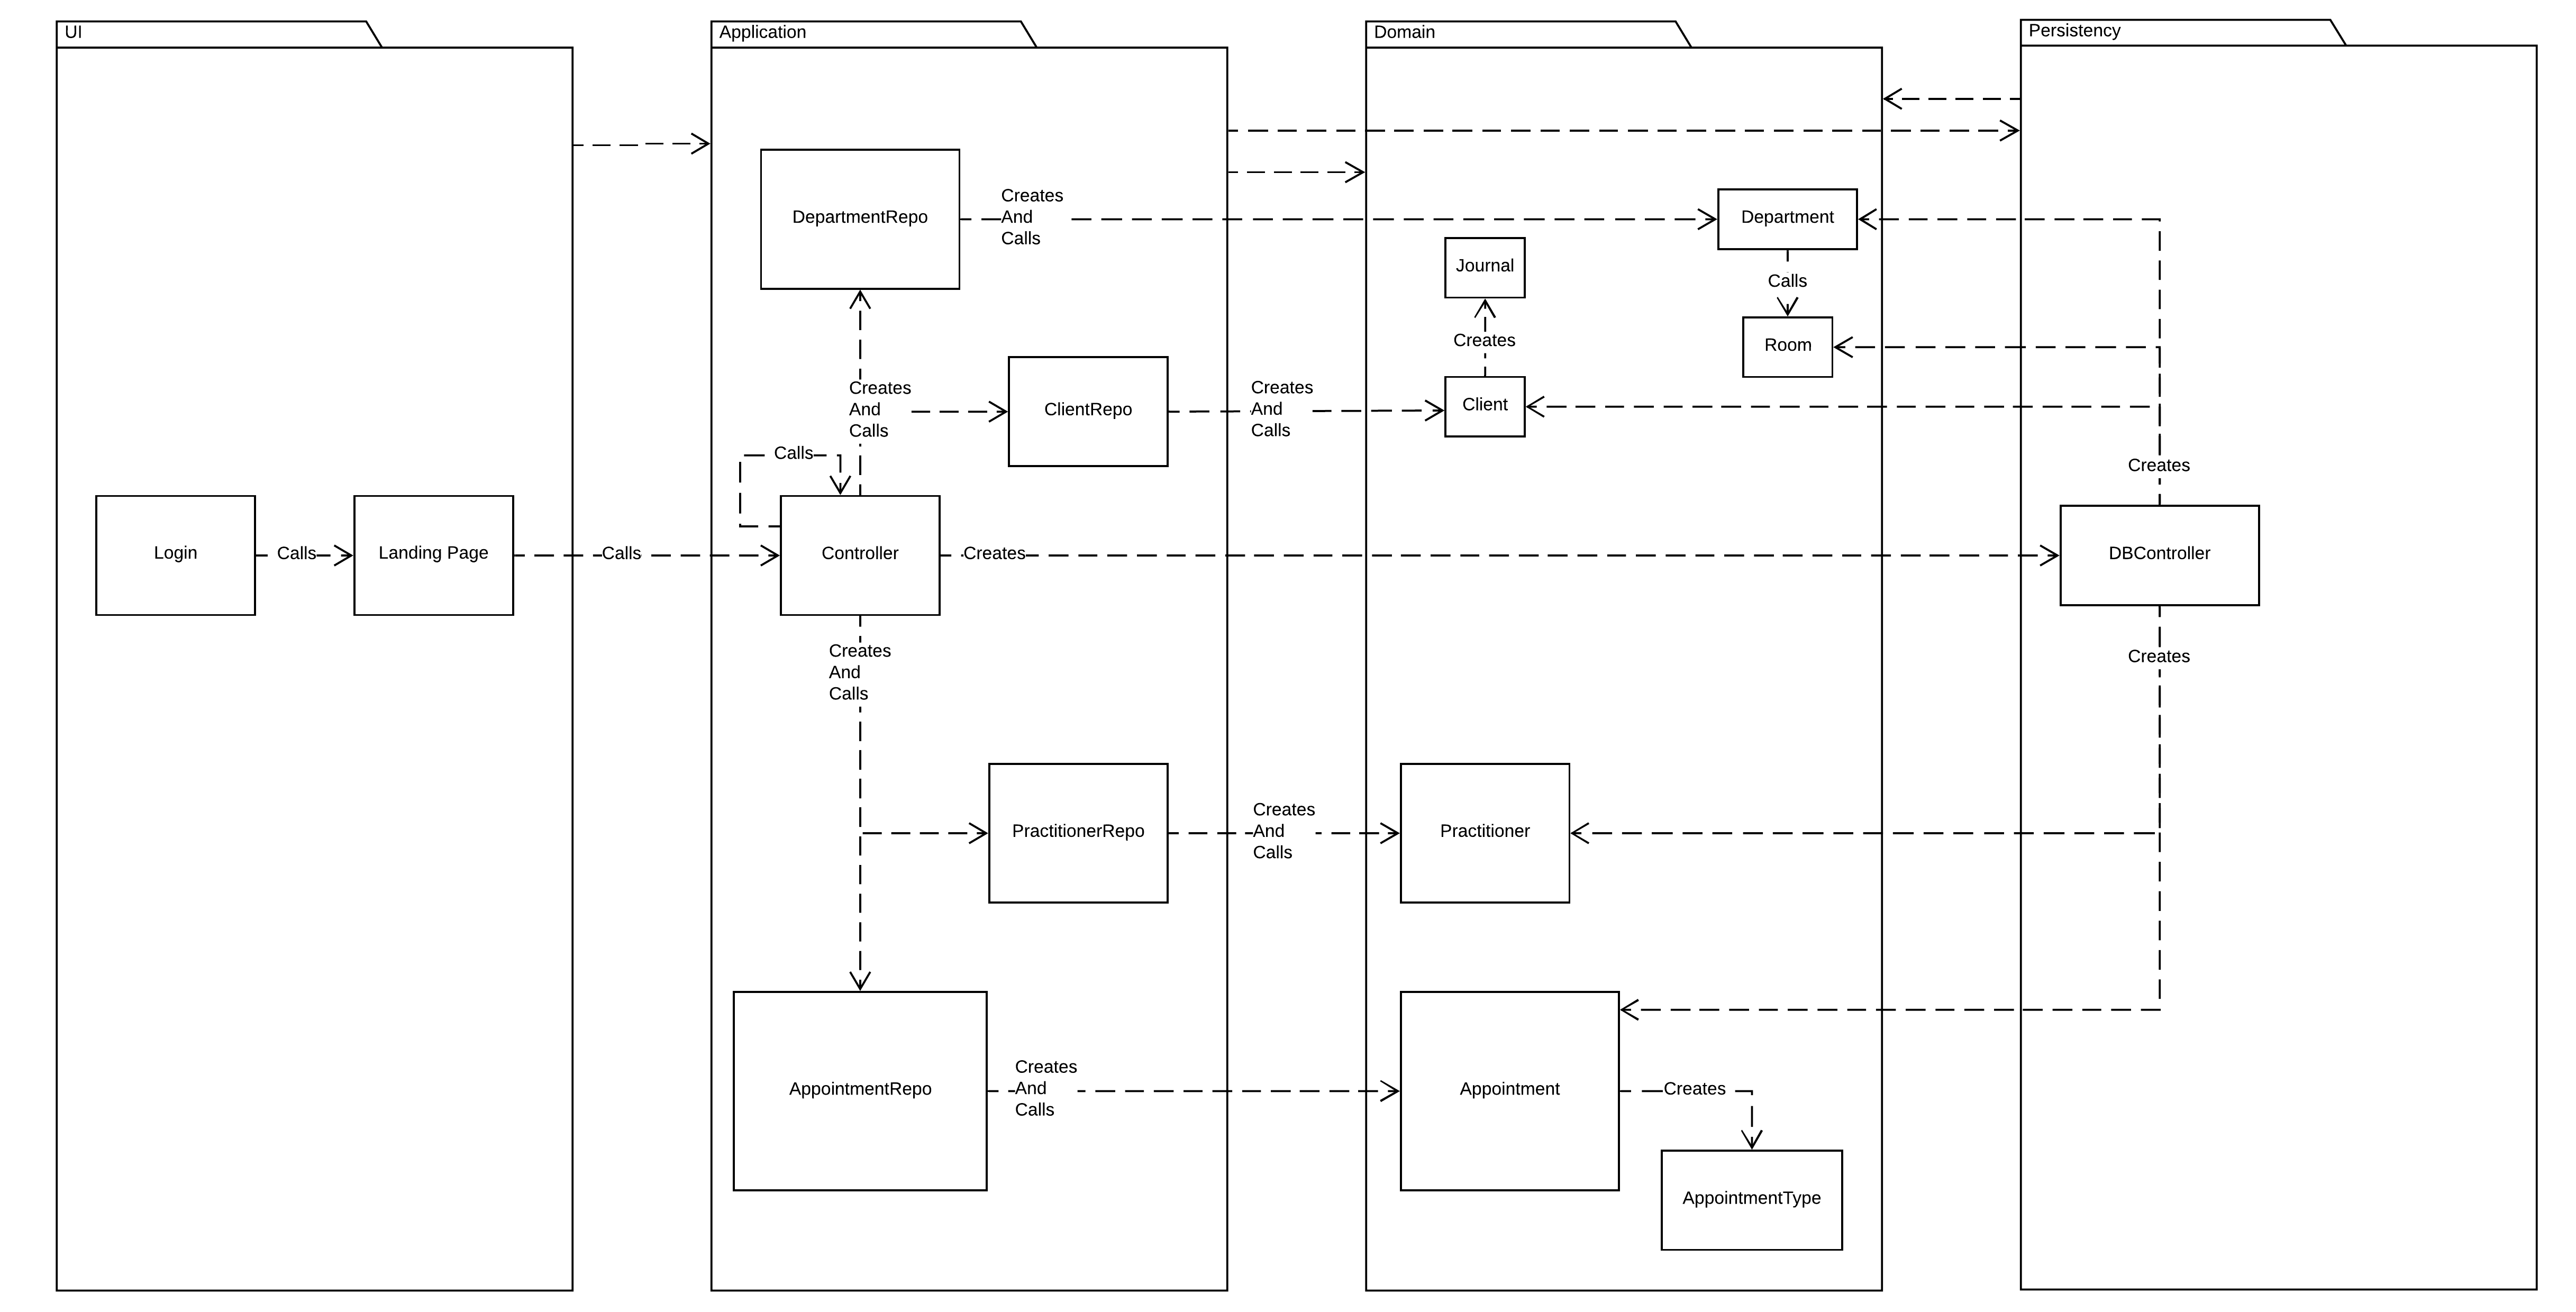
\includegraphics[width=\textwidth]{Pakkediagram.png}
    \label{fig:pakkediagram}
\end{sidewaysfigure}

\section{Modellering af Semplitos database(DBD)}
\label{kabitel:ModelleringDB}
\subsection{Databasediagram}
\label{DBD}


Vi har også opstillet et DBD, for at bedre overskue opstillingen af databasen.
Opstillingen af DBD'et er gjort med udgangspunkt i vores domænemodel og DCD.
Ved at betragte domænemodellen og diskutere hvilke domæneklasser, der vil være nødvendige at kunne tilgås for alle brugere af systemet ligegyldigt hvor og hvornår de er, har vi designet DBD'et som kan ses på figur \ref{fig:DBD}.

Diagrammet i sig selv har været til stor hjælp, især ved normalisering af vores tabeller. 

\begin{figure}[H]
    \caption{Databasediagram for systemet}
    \centering
        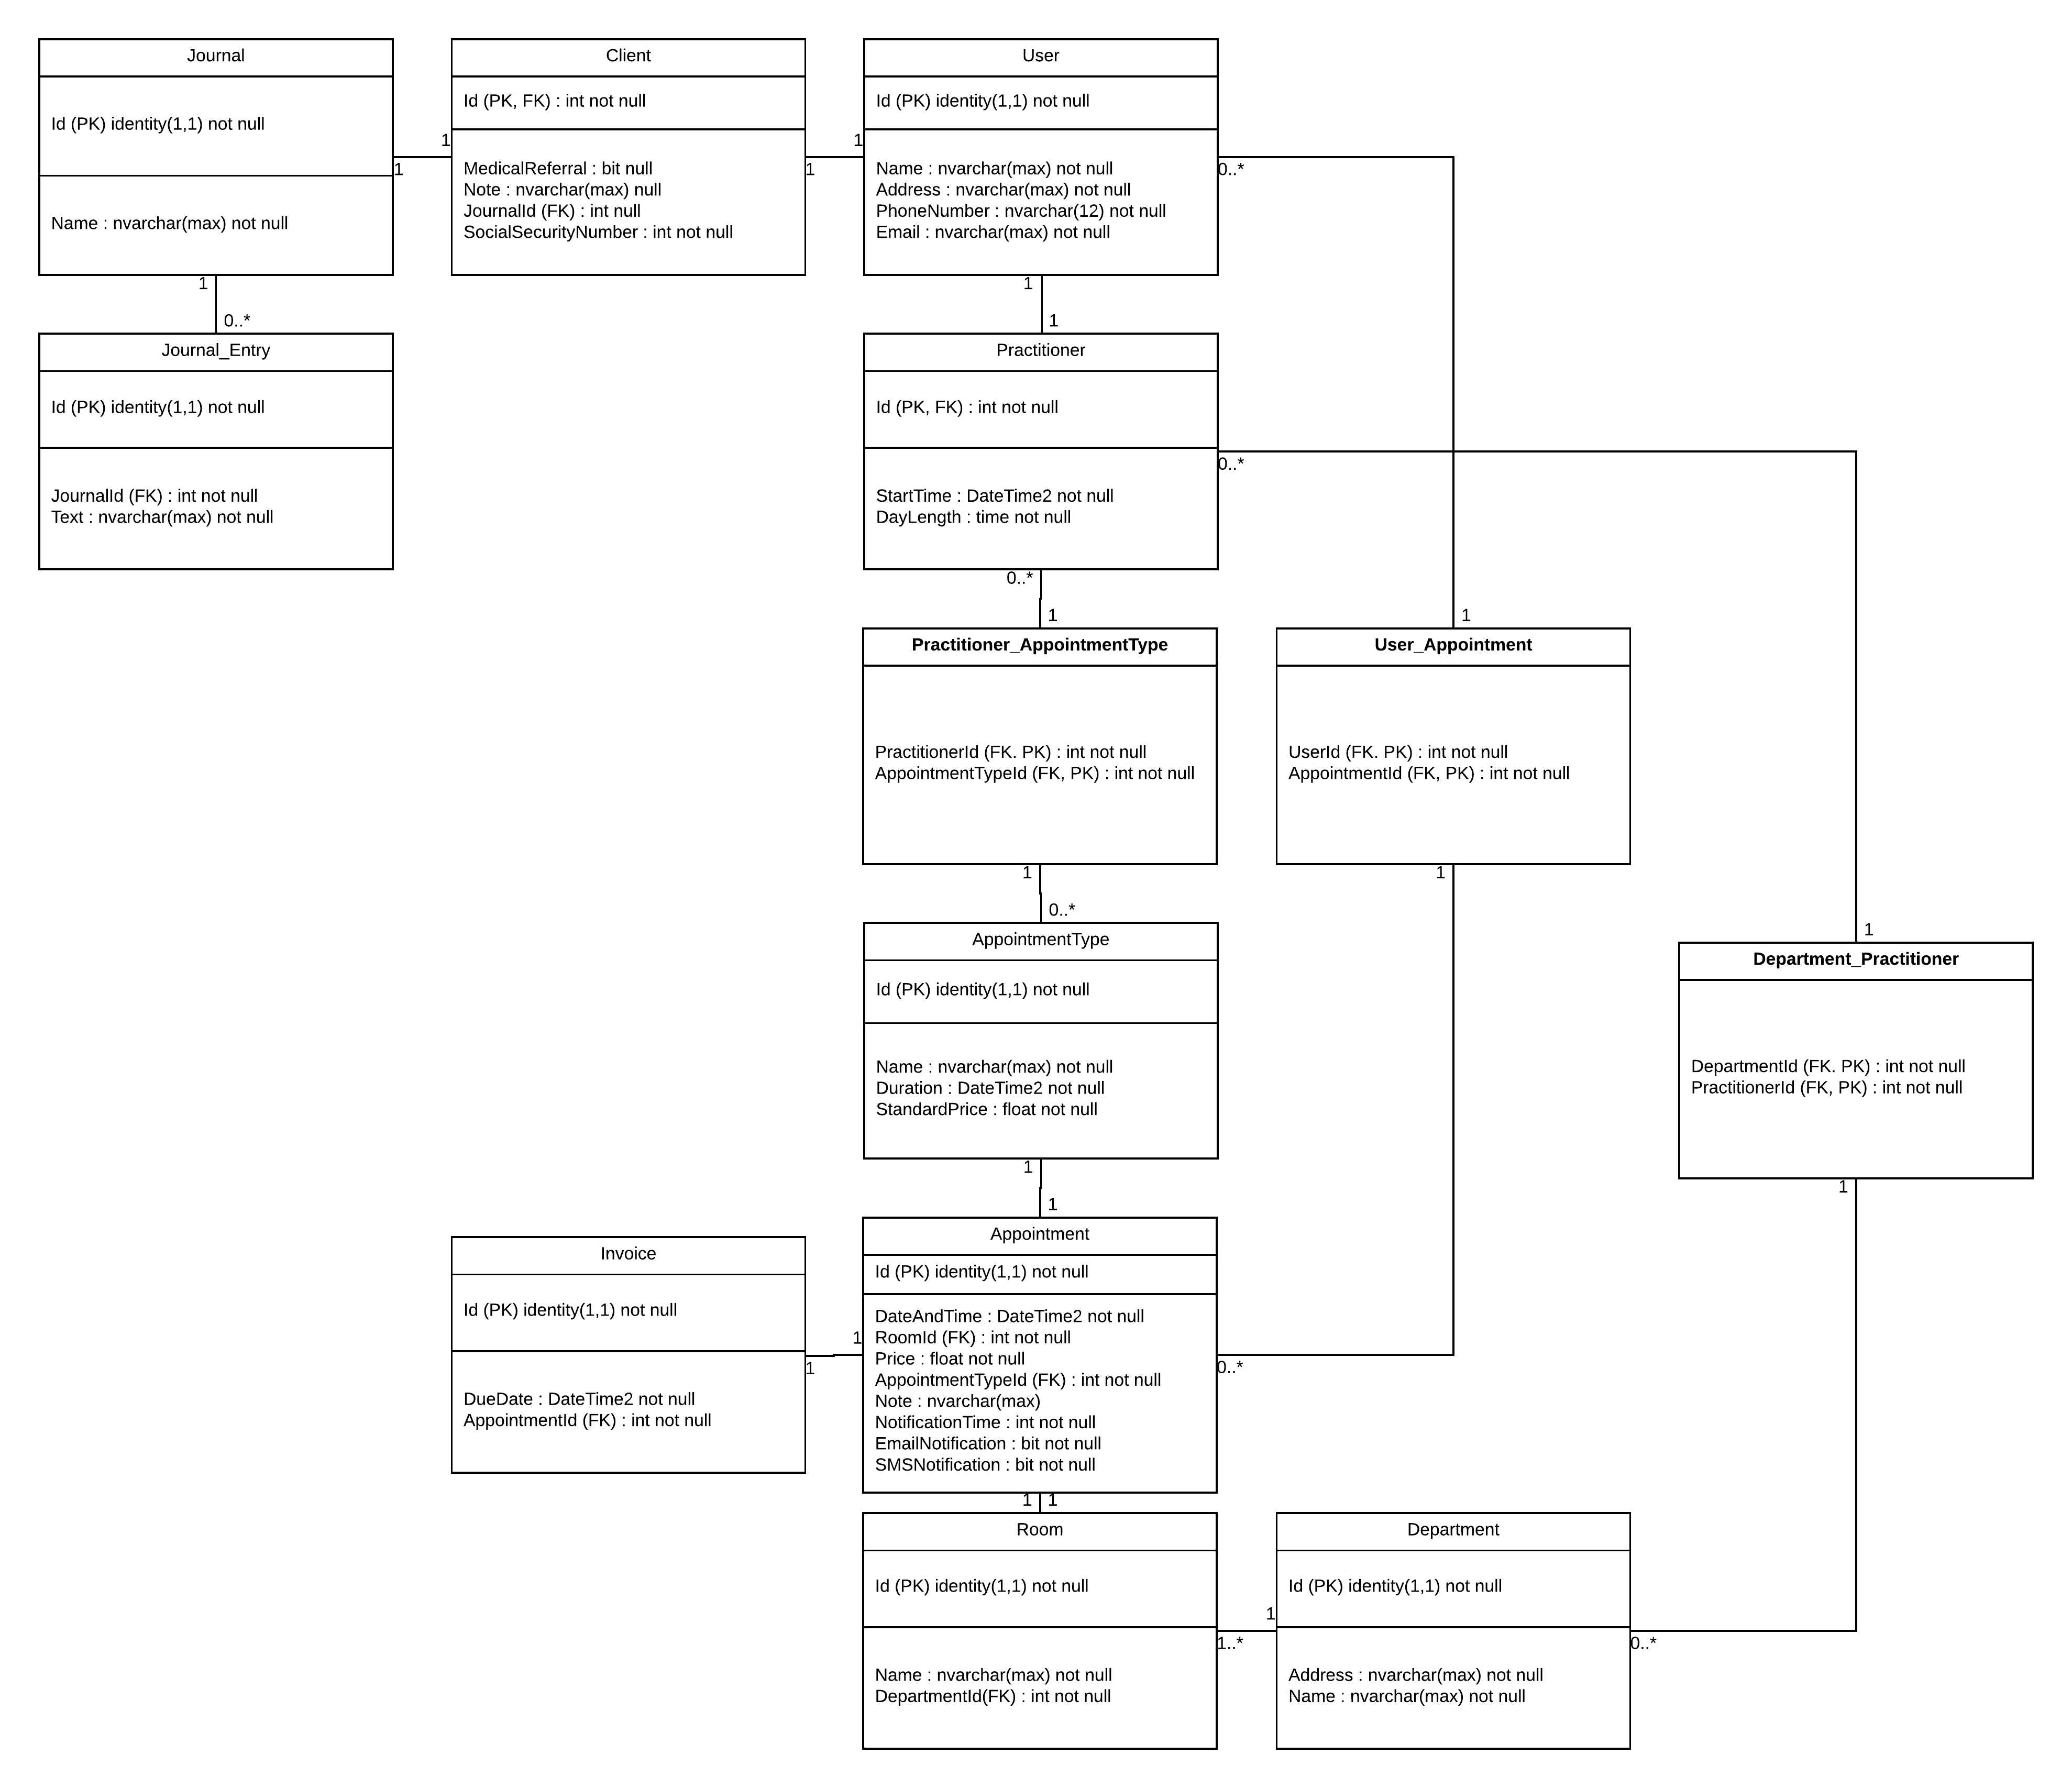
\includegraphics[width=\textwidth]{DBD.png}
    \label{fig:DBD}
\end{figure}

\subsubsection{Relationel database}

Vi har valgt at bruge en relationel database; hvor alt data er repræsenteret som tupler grupperet i relationer.
Den relationelle model blev først beskrevet af Edgar F. Codd i 1969.
Vi har valgt at bruge denne type af database, da vi har mange domæneklasser, der har forskellige sammenhænge, som det kan ses på figur \ref{system:domaene}.

Hvis vi blot havde vores database som en lang liste af data ville det give problemer.
Man kan forestille sig, at PsykologNord ansætter en ny behandler, som endnu ikke har nogen aftaler.
Det ville betyde, at vi ville have en masse tomme værdier i resten af den række, hvor behandlerens informationer står.\cite{database}

I stedet deles den store tabel op i mindre tabeller, der indeholder referencer til hinanden.

\subsubsection{Normalisering af databasediagrammet}

Hvor mange forskellige tabeller skal man så lave? Til at finde ud af dette bruger man det, som Codd kalder normalformer.
Der eksistere et hav af normalformer, men i denne rapport vil der arbejdes med første, anden, tredje og Boyce-Codd normalform.

Man bruger normalisering og normalformerne til at reducere redundans og forbedre præcisionen og konsistens af dataene i ens database.

Første normalform er opfyldt, når følgende gælder:
\begin{itemize}
    \item Alle cellerne i en tabel indeholder én værdi
    \item Alle indgange i en søjle er af samme type
    \item Hver søjle har et unikt navn
    \item Rækkefølgen af søjlerne er ligegyldig
    \item Rækkefølgen af rækkerne er ligegyldig
    \item Ingen rækker er ens
\end{itemize}

Anden normalform er opfyldt, når første normalform er opfyldt, og når det gælder, at alle ikke primærnøgle søjler er afhængig af \textit{hele} primærnøglen og ikke kun en del af primærnøglen.
Det betyder altså, at det kun er tabeller med sammensatte primærnøgler, der kan være på første normalform uden også at være på anden normalform. Hvis man har en tabel \textbf{(\underline{A}, \underline{B}, C, D, E)}, hvor \textbf{(A, B)} er en sammensat nøgle, skal det altså gælde at \textbf{C}, \textbf{D} og \textbf{E} ikke kan bestemmes af kun \textbf{A} eller kun \textbf{B}.

En tabel er på tredje normalform, hvis den er på anden normalform og der er ingen funktionelle afhængigheder i mellem ikke-nøgle søjler.
Det betyder altså, at hvis vores ovenstående eksempel skal være på tredje normalform må ingen af \textbf{C}, \textbf{D} eller \textbf{E} kunne bestemmes af \textbf{C}, \textbf{D}, \textbf{E} eller en kombination af disse.

For at opnå Boyce-Codd normalform skal tabellen være på tredje normalform, og alle determinanter skal være kandidatnøgler.
En determinant er den frie variable i en funktionel afhængighed. Har man funktionen \(f(n) = 5n^2 \), vil \(n\) være determinanten.\cite{database}

Måden vi har normaliseret vores database er ved først at identificere alle funktionelle afhængigheder, og så opstille tabeller, så alle determinanter er kandidatnøgler.
De er ikke alle primærnøgler, da vi har valgt at bruge substitutnøgler som primærnøgler.

Vores databasediagram kan ses på figur \ref{fig:DBD}.

\subsubsection{Views}

Et view er en virtuel tabel, hvis indhold defineres ud fra en forespørgsel.
Et view kan bruges som et filter til databasen, så man kan bestemme, hvordan hver enkelte bruger ser databasen.
Desuden kan det også bruges til at samle flere databaser og præsentere dem til brugeren som én database.

Vi bruger ikke på nuværende tidspunkt views i vores database, men det kunne have været fordelagtigt, at de stored procedures vi bruger til at hente informationer fra databasen hentede data fra views i stedet for at hente data direkte fra databasen.
Hvis vi ændrer databaseopbygningen nu, skal vi også ændre vores stored procedures og muligvis også vores kode i vores program, hvor hvis vi brugte views ville vi blot skulle ændre viewet, så det præsenterer dataene på samme måde som inden ændringen i databasen.

\subsubsection{Stored Procedures}
En stored procedure (SP) er gemt SQL forespørgsler, så det nemt kan køres igen, når det skal bruges.
Man kan bruge stored procedures til at bestemme, hvordan en bruger kan interagere med ens database ved at sætte rettighederne så brugeren kun kan køre allerede eksisterende stored procedures.
Det er blevet lavet forskellige SP'er primært ud fra CRUD princippet og de vi har brugt i vores system kan ses i figur \ref{StoredProcedures}

\begin{figure}[h]
    \caption{Stored Procedures}
    \centering
        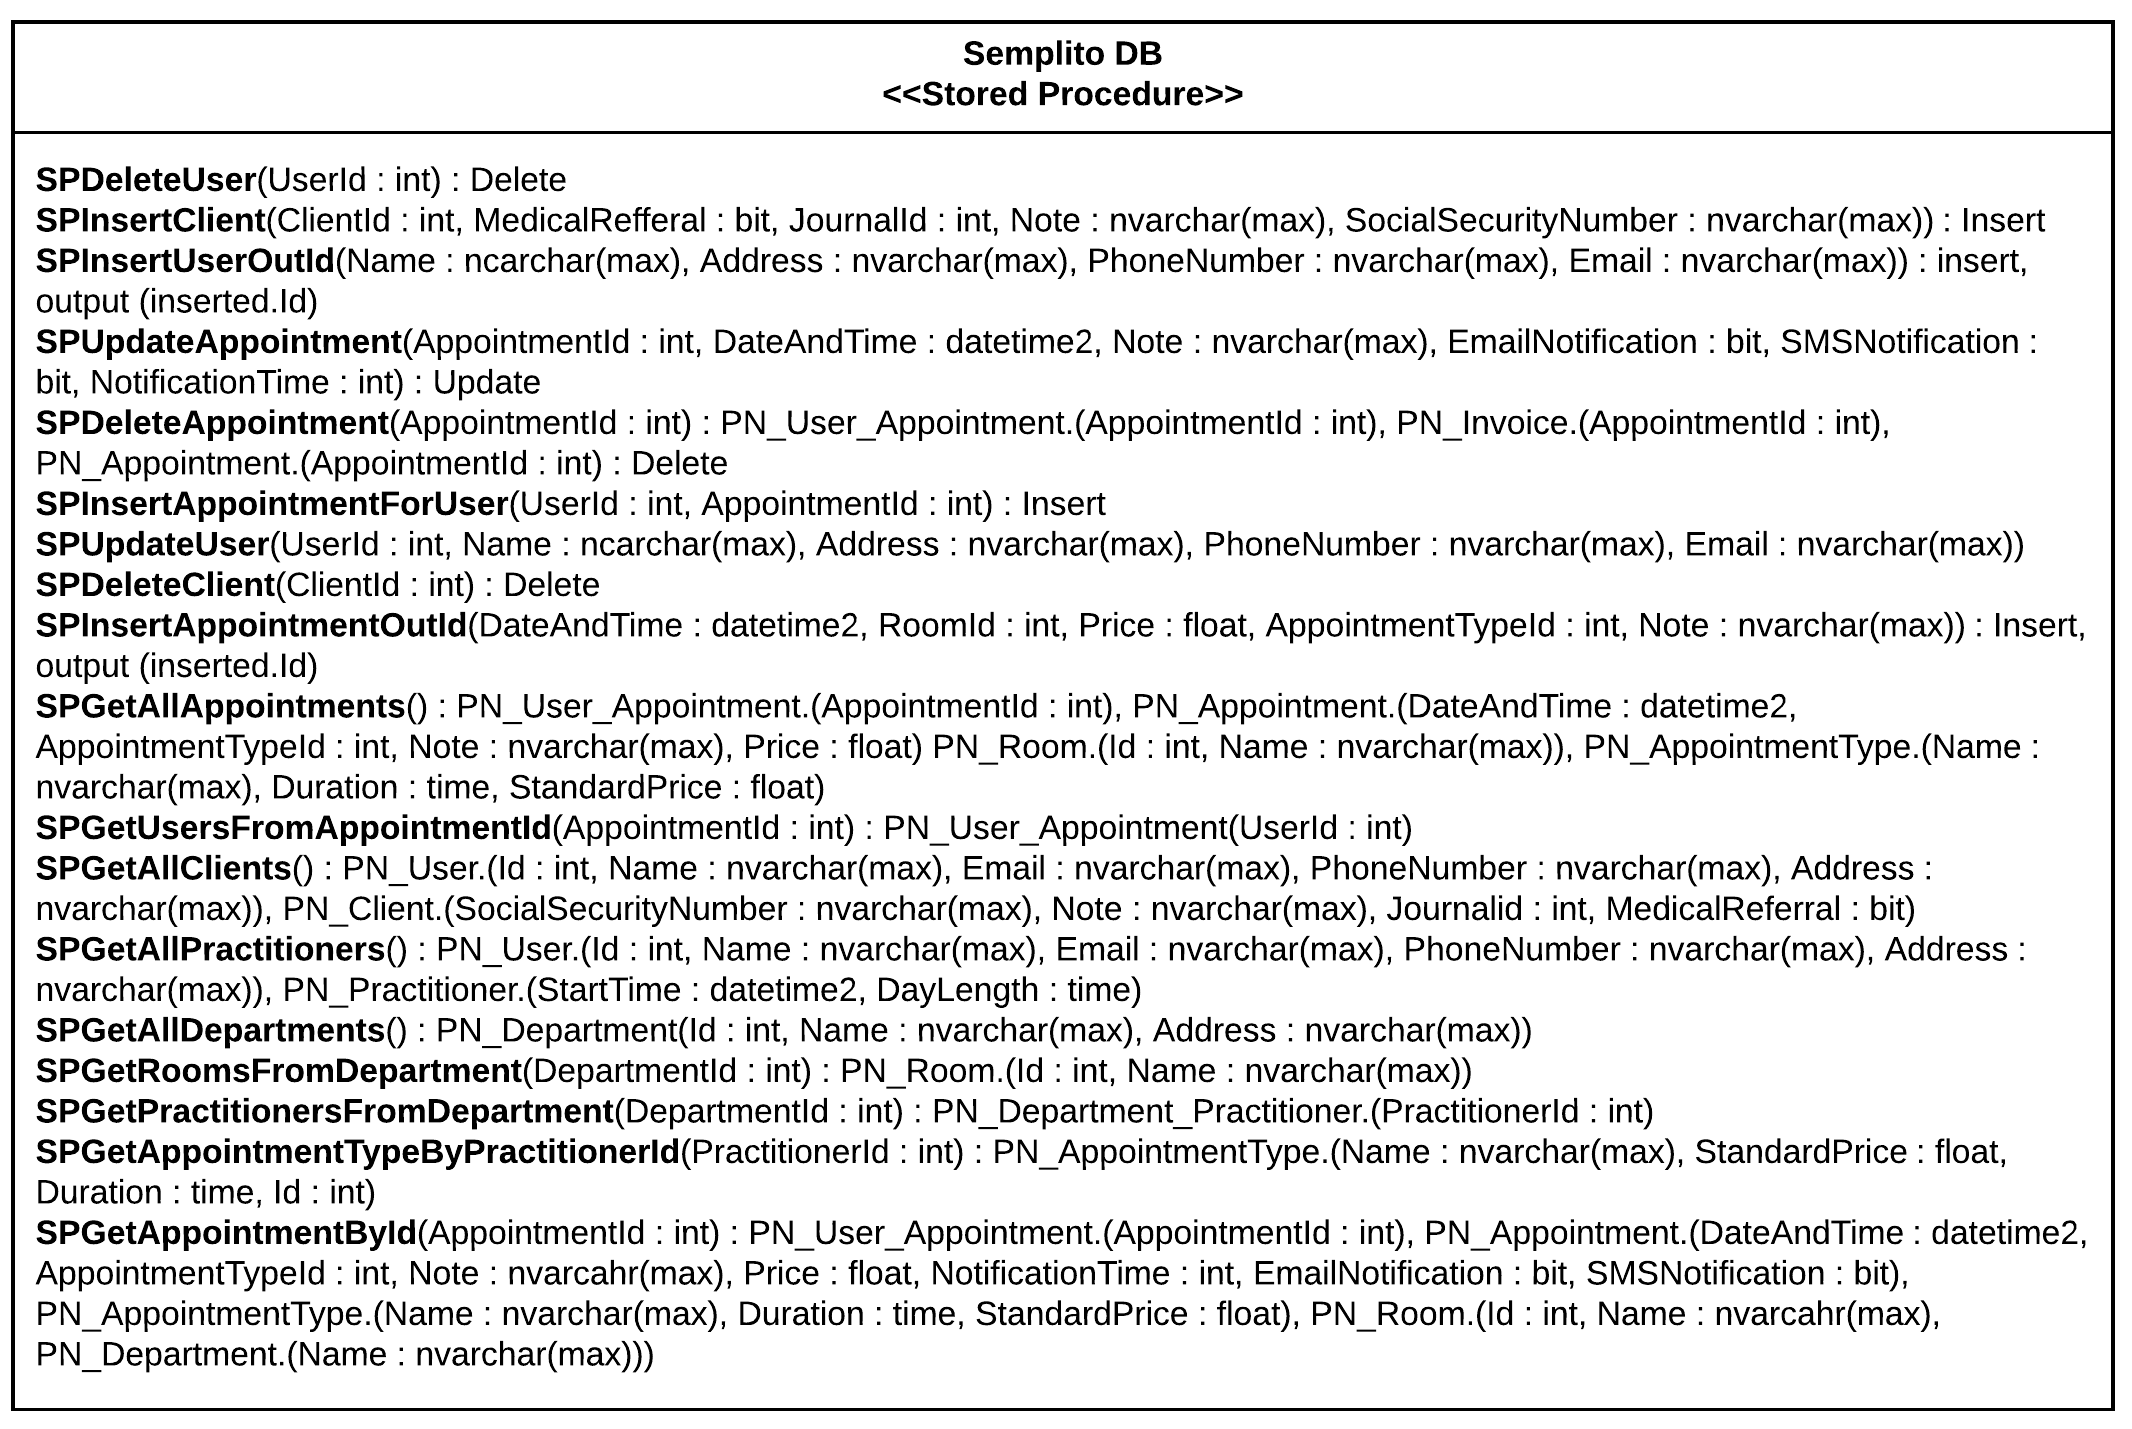
\includegraphics[width=\textwidth]{SP.png}
    \label{StoredProcedures}
\end{figure}

Vi har valgt at beskrive SP'en SPGetAllAppointments, se figur \ref{SPGetAllAppointments}, for at vise hvordan man kan bruge JOIN til at hente fra flere forskellige tabeller og få et enktelt table som output.

\begin{figure}[h]
    \caption{SPGetAllAppointments}
    \centering
        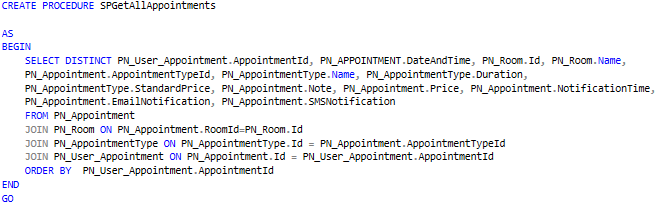
\includegraphics[width=\textwidth]{SPGetAllAppointments.png}
    \label{SPGetAllAppointments}
\end{figure}

Der er blevet brugt SELECT DISTINCT, som sørger for at der ikke er nogle duplicationer af data i outputted. Vi brugte det som et debugging værktøj, hvor det ikke er blevet fjernet fordi vi gerne ville være sikre på at der ikke var duplicationer.
+Der er blevet brugt fire JOIN's i denne SP, keyworded JOIN i MSSQL er i sig selv et LEFT JOIN dvs. at den tager alt fra den første table og forener på det de har tilfælles. Det gøres ved keyworded ON hvor der efter bliver lavet en sammenligning på deres PK og den modsatte tables FK.
Tilsidst er der blevet brugt ORDER BY, som sørget for at den kommer i den rækkefølge som vi gerne vil have det i.
